\subsection{Discrete-time Baseband Wireless communication Model}

The general discrete-time baseband wireless communication model is illustrated in Fig.\ref{fig:wireless-system-model}, which consists of three 
parts: transmitter, wireless channel, and receiver.

\begin{figure}[htbp]
  \centering
  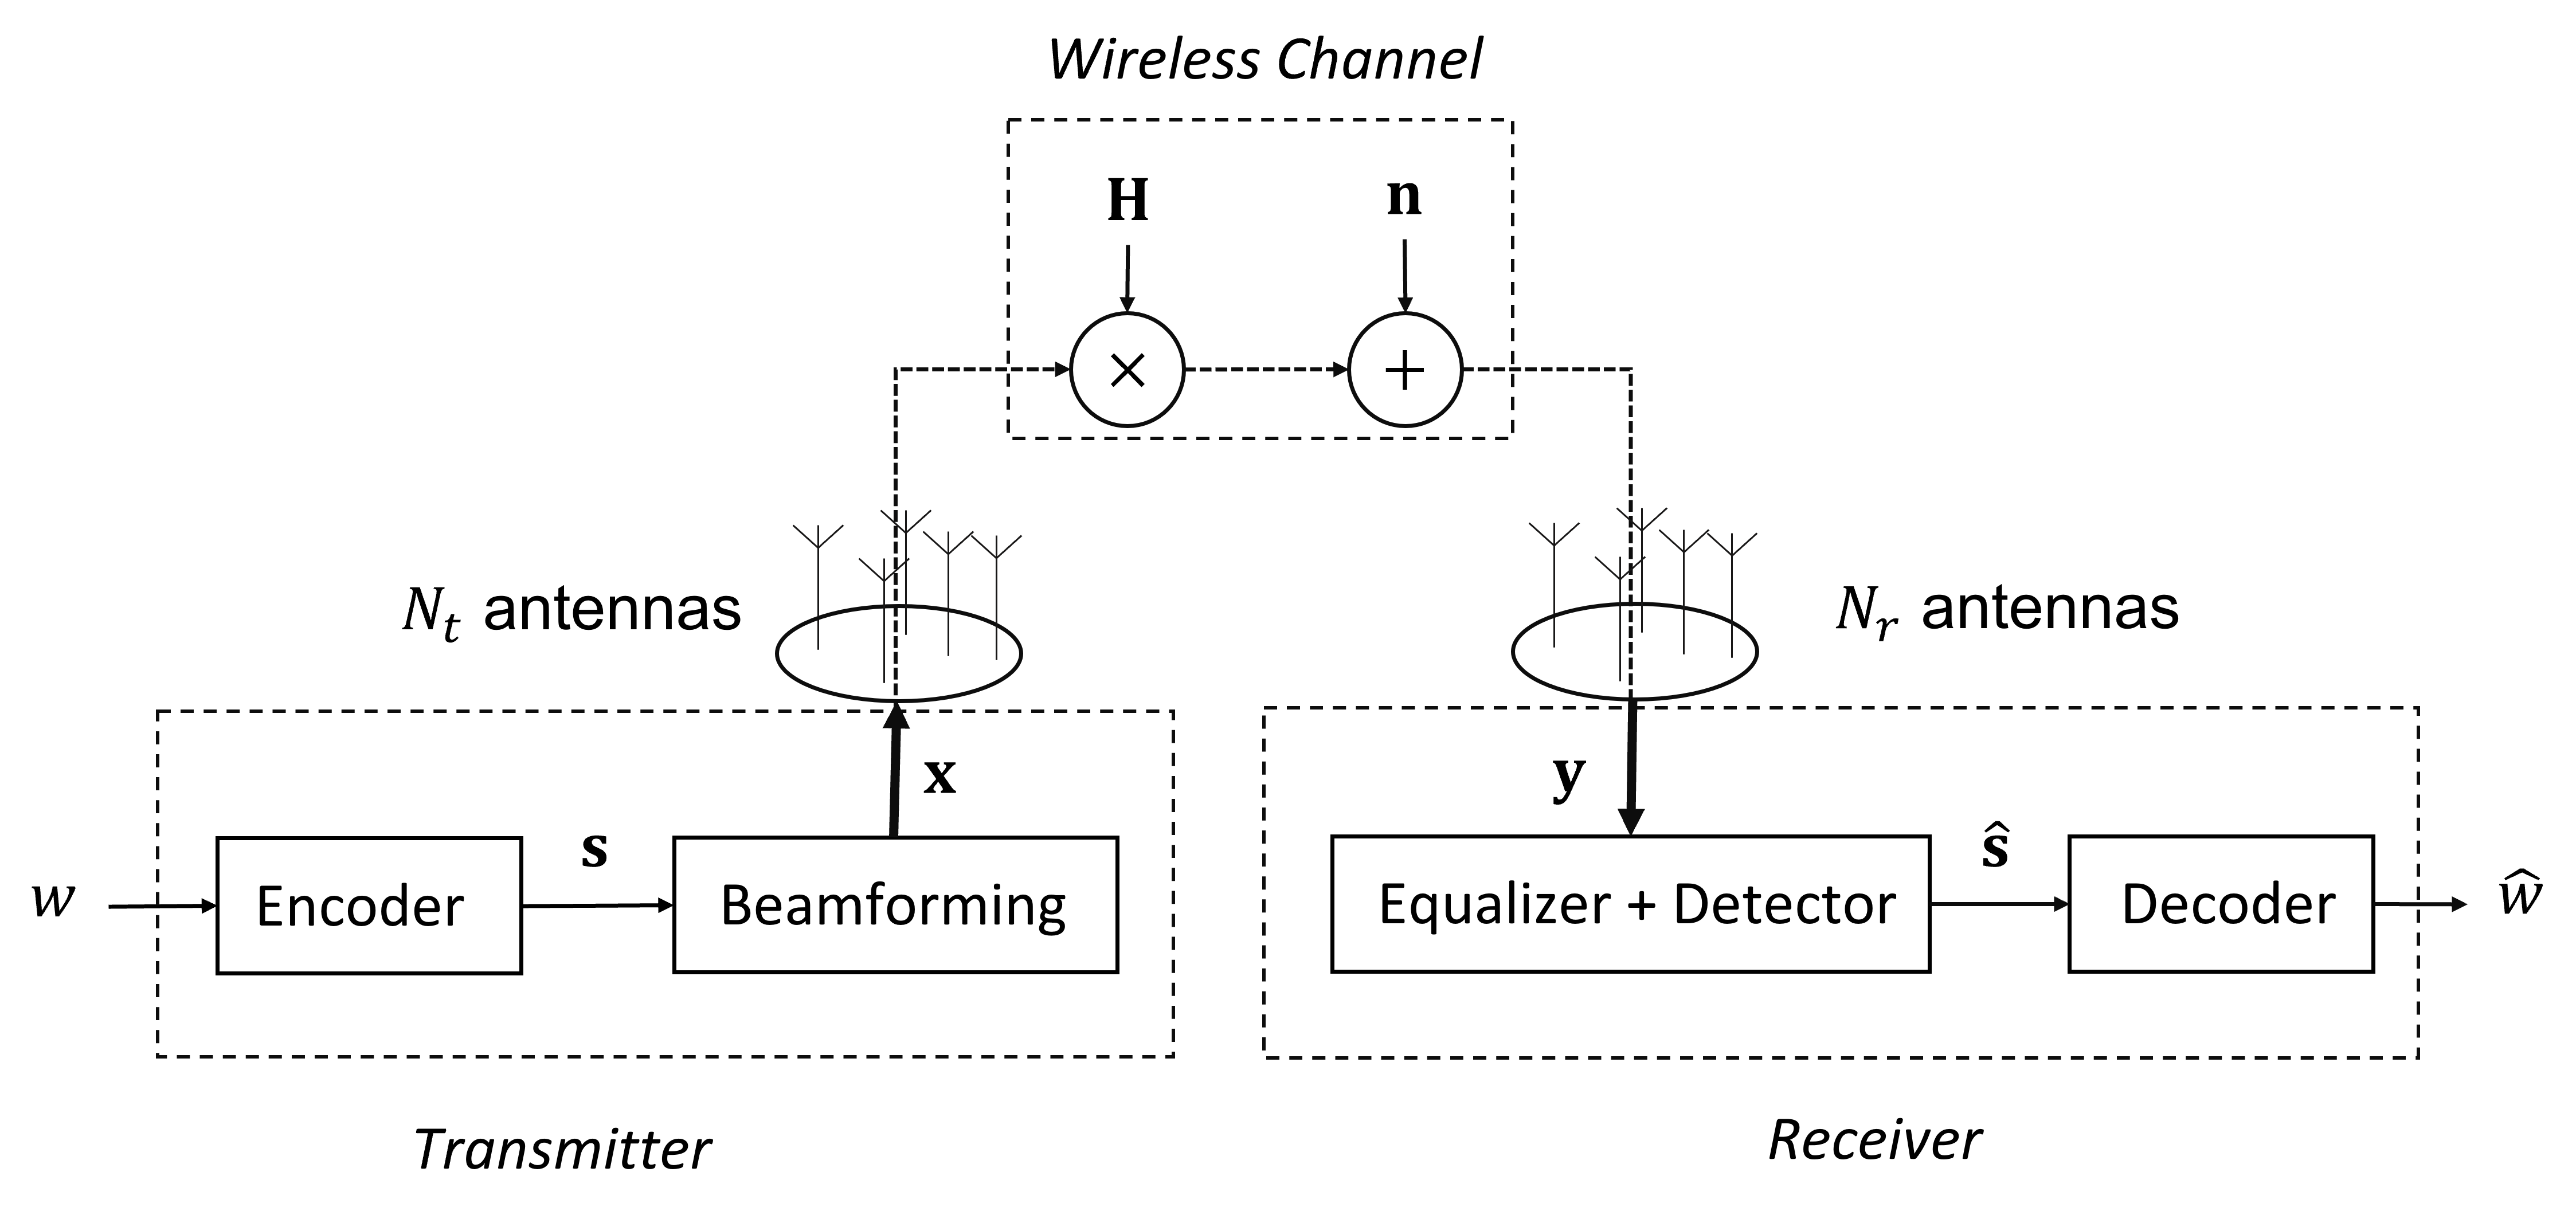
\includegraphics[width=1.0\textwidth]{./wireless-system-model.png}
  \caption{General discrete-time baseband wireless communication model}
  \label{fig:wireless-system-model}
\end{figure}

The wireless communication systems can be classified into:
\begin{itemize}
    \item SISO (Single-Input Single-Output): $N_t=N_r=1$;
    \item SIMO (Single-Input Multiple-Output): $N_t=1, N_r > 1$;
    \item MISO (Multiple-Input Single-Output): $N_t>1, N_r=1$;
    \item MIMO (Multiple-Input Multiple-Output): $N_t>1, N_r>1$. 
\end{itemize}

Let's firstly take SISO as an example. Without considering noise, the wireless channel is modeled as \cite{tse2005fundamentals}
\begin{equation}
    h(\tau, t) = \sum_i \beta_i(t) \delta(\tau - \tau_i(t)),
\end{equation}
where $h(\tau, t)$ is the channel response at time $t$ to an impulse transmitted at time $t-\tau$. Thus, the received signal
for the transmitted $c(t)$ is
\begin{align}
    y(t) &= \int_{-\infty}^{\infty} h(\tau,t) c(t-\tau) d\tau \nonumber \\
    &= \sum_i \beta_i(t) c(t-\tau_i(t)).
\end{align}
Since many operations in wireless communication system are at baseband, we usually transform the signal to baseband. The baseband
equivalent of $y(t)$ is \cite{tse2005fundamentals}
\begin{equation} \label{eqn:baseband_equivalent}
    y_b(t) = \sum_i \beta_i^b c_b(t-\tau(t)),
\end{equation}
where $\beta_i^b(t) = \beta_i(t) e^{-j2\pi f_c \tau_i(t)}$ with $f_c$ denoting carrier frequency. $c_b(t)$ is the baseband equivalent of 
$c(t)$ and is defined as
\begin{equation}
    c_b(t) = \frac{1}{\sqrt{2}}\Big(c(t) + \hat{c}(t)\Big) e^{-j2\pi f_c t},
\end{equation}
where $\hat{c}(t)$ is the Hilbert transform of $c(t)$. Thus, according to \eqref{eqn:baseband_equivalent}, the baseband channel response is
\begin{equation}
    h_b(\tau, t) = \sum_{i} \beta_i^b \delta(\tau - \tau_i(t)).
\end{equation}
For a digital system, the signal need to be sampled. From Shannon sampling theorem, if $c_b(t)$ is band-limited to $B/2$, it
can be transformed as
\begin{equation} \label{eqn:shannon_transform_of_received_signal}
    c_b(t) = \sum_n c[n] {\rm sinc} (Bt - n),
\end{equation}
where $c[n] = c_b(n/B)$ is the sampled version of $c_b(t)$. By substituting \eqref{eqn:shannon_transform_of_received_signal}
into \eqref{eqn:baseband_equivalent}, we have
\begin{equation}
    y_b(t) = \sum_n c[n] \sum_i \beta_i^b(t) {\rm sinc}(Bt - B\tau_i(t) -n).
\end{equation}
The sampled version of $y_b(t)$ with $f_s = B$ is
\begin{align}
    y[k] & \coloneqq y_b\left( \frac{k}{B} \right) \nonumber \\ 
    & = \sum_n c[n] \sum_i \beta_i^b \left( \frac{k}{B} \right) \mathrm{sinc} \left[ k-n-B\tau_i\left( \frac{k}{B} \right) \right] \nonumber\\ 
    & \stackrel{\ell=k-n}{=} \sum_\ell c[k-\ell] \sum_i \beta_i^b \left( \frac{k}{B} \right) \mathrm{sinc} \left[\ell - B\tau_i \left( \frac{k}{B} \right) \right]
\end{align}
Therefore, the discrete-time baseband equivalent of channel response is 
\begin{equation}
    h_\ell[k] = \sum_i \beta_i^b \left( \frac{k}{B} \right) \mathrm{sinc} \left[ \ell- W \tau_i\left( \frac{k}{B} \right) \right].
\end{equation}
By considering the additive noise, the discrete-time baseband system model of wireless communication system is
\begin{equation}
    y[k] = \sum_\ell h_\ell[k]c[k-\ell] + n[k].
\end{equation}
In flat fading, the channel is represented by a single channel filter tap \cite{tse2005fundamentals}
\begin{equation}
    y[k] = h[k]c[k] + n[k].
\end{equation}

We now expand the SISO case to a general one. By dropping the time index, the received signal for any amounts of antennas is
\begin{equation}
    {\bf y} = {\bf H} {\bf c} + {\bf n},
\end{equation}
where ${\bf y} \in \mathbb{C}^{N_r \times 1}$, ${\bf H} \in \mathbb{C}^{N_r \times N_t}$, ${\bf c}\in \mathbb{C}^{N_t \times 1}$,
and ${\bf n} \sim \mathcal{CN}({\bf 0}, \sigma_n^2 {\bf I}_{N_r})$.

When $N_t > 1$, beamforming, also called linear precoding, is usually exploited to eliminate the interference on 
each independent stream $s_i \in \mathbb{C}, i=1,...,R$ in the transmitted ${\bf s}$, by adjusting the gain and phase of the signal fed to each antenna.
The beamforming matrix is denoted by ${\bf P} = [{\bf p}_1,...,{\bf p}_R] \in \mathbb{C}^{N_t \times R}$. The received signal 
can be rewritten as
\begin{equation} \label{eqn:wireless-received-signal-beamforming}
    {\bf y} = {\bf HPs + n} = {\bf H}\sum_{i=1}^R {\bf p}_is_i + {\bf n},
\end{equation}
where $R \leq {\rm rank}({\bf H})$ and ${\rm Tr}({\bf PP}^H) \leq P_t$. $P_t$ is the power budget of transmitter.

At the receiver, the equalizer can also be used to minimize the interference. Let ${\bf g}_j \in \mathbb{C}^{1 \times N_r}$
denote the equalizer for $j$-th stream. The input of detector is given as
\begin{equation}
    z_j = {\bf g}_j{\bf H}\sum_{i=1}^R {\bf p}_is_i + {\bf g}_j {\bf n}.
\end{equation}
Then, $\hat{s}_j$ is detected by the detector based on $z_j$.


\subsection{Capacity of Wireless Channels}
Capacity or achievable rate is one of the most representative metrics of a wireless communication system and gives the upper bound 
of the data rate that can be transmitted in a specific channel without any error.

The transmitted signal $\sqrt{E_s}x$ through additive white Gaussian noise (AWGN) channel is
\begin{equation}
    y = \sqrt{E_s}x + n,
\end{equation}
where $E_s$ is transmit power, $x$ satisfies $\mathbb{E}(|x|^2)=1$ and $n \sim \mathcal{CN}(0,\sigma_n^2)$ is complex Gaussian noise.
The AWGN channel capacity can be derived by Shannon information theory and is given as
\begin{equation}
    C = \log_2 (1+\rho) \quad [{\rm bits/s/Hz}],
\end{equation}
where $\rho = E_s/\sigma_n^2$ is the signal-to-noise ratio (SNR).

However, in fading channel, the capacity is also determined by fading. The capacity in different fading is shown as follows \cite{clerckx2013mimo}:
\begin{itemize}
    \item \textbf{Deterministic SISO Channel}
    
    \begin{align}
        &\text{Received signal: } y = \sqrt{E_s} h c + n \\
        &\text{Capacity: } C = \log_2(1+\rho|h|^2) \quad [\mathrm{bits/s/Hz}]
    \end{align}
    
    % \noindent Received signal: $y = \sqrt{E_s} h c + n$

    % \noindent Capacity: $C = \log_2(1+\rho|h|^2) \quad [\mathrm{bits/s/Hz}]$
    
    \item \textbf{Deterministic SIMO Channel}
    
    \begin{align}
        &\text{Received signal: } {\bf y} = \sqrt{E_s} {\bf h} c + {\bf n} \\
        &\text{Capacity: } C = \log_2(1+\rho\|{\bf h}\|^2) \quad [\mathrm{bits/s/Hz}]
    \end{align}
    In SIMO channel, the capacity can be achieved by maximum ratio combination (MRC) at receiver, i.e.,
    \begin{equation}
        {\bf h}^H {\bf y} = \sqrt{E_s} \|{\bf h}\|^2 c + {\bf h}^H {\bf n}
    \end{equation}

    \item \textbf{Deterministic MISO Channel}
    
    \begin{align}
        &\text{Received signal: } y = \sqrt{E_s} {\bf h} {\bf w}c + n \\
        &\text{Capacity: } C = \log_2 (1+\rho\|{\bf h}\|^2) \quad [\mathrm{bits/s/Hz}]
    \end{align}
    In MISO channel, the capacity can be achieved by maximum ratio transmission (MRT) with perfect transmit channel knowledge, i.e.,
    ${\bf w} = {\bf h}^H/\|{\bf h}\|$ and   
    \begin{equation}
        y = \sqrt{E_s} \|{\bf h}\| c + n
    \end{equation}

    \item \textbf{Deterministic MIMO Channel}

    \begin{align}
        &\text{Received signal: } {\bf y} = \sqrt{E_s} {\bf H} {\bf c}' + {\bf n}\\
        &\text{Capacity: } C = \max_{{\bf Q} \ge 0: \mathrm{Tr}\{{\bf Q}\}=1} \log_2 \det\left[ {\bf I}_{N_r} + \rho {\bf HQH}^H\right] \quad [\mathrm{bits/s/Hz}]
    \end{align}
    where ${\bf Q} = \mathbb{E}({\bf c}'{\bf c}'^H)$ is the covariance of transmitted signal. The capacity can be achieved by applying 
    multiple eigenmode transmission and using water-filling algorithm to find the optimal ${\bf Q}^\star$.

\end{itemize}

% \begin{table}[h!]
%     \caption{Channel capacity in different communication system}
%     \centering
%     \begin{tabular}{llll}
%             System    & Received Signal                               & Capacity                                 & Realization                             \\ \hline                                   
%             SISO      & $y = \sqrt{E_s} h c + n_k$                    & $C = \log_2(1+ \rho|h|^2)$               &                                         \\
%             SIMO      & ${\bf y} = \sqrt{E_s} {\bf h} c + {\bf n}_k$  & $C = \log_2(1+\rho\|{\bf h}\|^2)$        & MRC receiver ${\bf g} = {\bf h}^H$      \\
%     \end{tabular}
%     \label{tab:reference_parameters}
% \end{table}